\section{System Description}\label{sec:system-description}

\subsection{Database}\label{sec:database}

\subsubsection{Schema and Indexes}\label{sec:schema-and-indexes}
The database schema was designed accordingly to the systems requirements. In the description of the system three main components can be clearly identified, the users, queues and messages. Taking those elements as base components of the system, the application works with three main tables in the database, each one corresponds to the main components in the system \( See Figure \ref{erd} \).\\

\begin{figure}[h!]
	\centering
	%\def \svgscale {\columnwidt}
	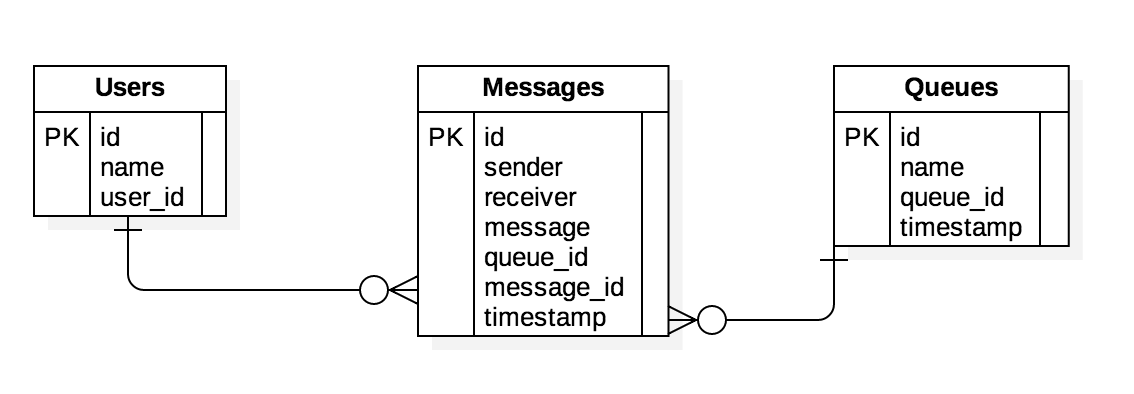
\includegraphics[width=\textwidth]{ERDDiagram1.png}
	\caption{Entity-Relation-Diagram of the database.}
	\label{erd}
	%\input{soft-mmu-2.pdf}
\end{figure}


The table user contains three columns. The id column is the auto increment value assigned from the database for each new row in the table. The column name contains the name of the users, this value is marked as unique, because each user must, have and a unique user name. Finally the userid column, is a second id that binds a user with the middleware and its assigned by it each time a new user connects to the system.\\

The table queue contains four columns. As in the previous table it has the id auto increment column. The column queuename, has the name of the queues in the database also marked as unique. The column queueid, also shares an id generated by the middleware, this value is assigned by the middleware when a users requests to create a new queue. Finally the column timestamps as the name implies, are the timestamps of the queue when this one is created.\\

The table messages, is the biggest but not necessarily complex table. Each column corresponds with each component of the message object. In the requirements is specified that each message must have a sender, receiver, the queue it belongs to, timestamp, the message content and the message id. Therefore, the table has a column for each of these parameters.\\

The indexes of the database are the following:\\
In the table users, there is a single index of the users, because that is the attribute used by the stored procedures to a find a particular user.\\
In the table queues, as in the previous table a single index is used to optimize the search over the id of the object queue.\\
Finally in the table messages, three indexes were created, one to search over the message id to find a particular message, an index to search over the receiver of a message, a use case of this index is when a user requests a message entitled to him a search over this value must be done. Lastly an index to search over the queid of which that message belongs, an example of the need of this index is when a user requests to delete a queue and all the messages stored in that queue must be found in order to eliminate them as well.


\subsubsection{Stored Procedures}\label{sec:stored-procedures}
The database messaging contains a total of 14 stored procedures, some created as testing tool and other as part of the functionality of the messaging system. A list of each store procedures in the system and a corresponding description of its function is presented next.\\

delete\_messages\_from\_queue(queue\_id): This functions are executed when user wants to delete a queue. Therefore each message that belongs to that queue is eliminated. This function expects the queue\_id value. The value is obtained by the get\_queue\_id(queue\_name) function.\\

delete\_queue(queue\_name): This function deletes a queue. However this cannot be done if there exist a message in the messages table that has on its queueid column the value of the id of the queue that is about to be deleted. This protection function is enabled as an initial relation established on the database.\\

delete\_user(user\_name): This function is on charge of deleting a user from the table users. Nevertheless, the database also has a protection mechanism regarding the messages on the database and the user id of the user that is about to be deleted. This constrained, stops the execution if there exists a message for this user.\\

get\_message(receiver\_name): This stored function retrieves a message for the corresponding receiver. If the message doesn’t exists it returns a empty message, with empty values on each column.\\

get\_message\_from(receiver\_n,sender\_n): This function gets a message from the database where the value of the sender and the receiver matches the ones passed as arguments to the function. If the message does not exist it returns an empty message, with empty values on each column.\\

get\_queue\_id(queue\_name): This function returns the id value of the queue specified in the name parameter. If the queue does not exists it returns empty.\\

get\_user\_id(user\_name): This function returns the user id of the user been requested. If the user does not exist it returns empty.\\

insert\_new\_queue(name,id,timestamp): This function is executed when a user requests the creation of a new queue. The queue name, the id created by the middleware and the timestamps of creation are provided as parameters to the function.\\

insert\_new\_user(name,id): This function is executed, when a new user connects to the middleware, in order to add this new user to the database. The name and the middleware id are provided in the function.\\

insert\_new\_message(message,sender,receiver,id,timestamps,queue\_id): This is the function executed when a user sends a new message to the database. The queue id is obtained using the get\_queue\_id(queue\_name) function and the return value depends on the name of the queue where the user want to allocate the message. The rest of the parameters are the default values of a normal new message.


\subsubsection{Design decisions}\label{sec:design-decisions}
The main goal during the design of the database was to comply with the system requirements in the system description. Furthermore once the requirements were fulfilled, I focused on a small schema in order to keep the size of the database small.\\
For the improvement of the operations on the database, the postgres functions (Stored procedures) were implemented.  Postgres functions written in PL/pgSQL execute the queries like prepared statements; they reused cache query plans, this make and improvement in the execution time, since they decrease the planning overhead for the execution.\cite{postsql}\\

In addition of the postgres functions also indexes were created in the database. Indexes improve the performance of the database specially when small amounts of data are expected to be retrieved. Since indexes on postgres are partially or totally cached accessing data form a cached source is always faster to access then from disk. This improves overall the performance of the database. 


\subsubsection{Performance characteristics}\label{sec:performance-characteristics}
\begin{figure}[h!]
	\centering
	%\def \svgscale {\columnwidt}
	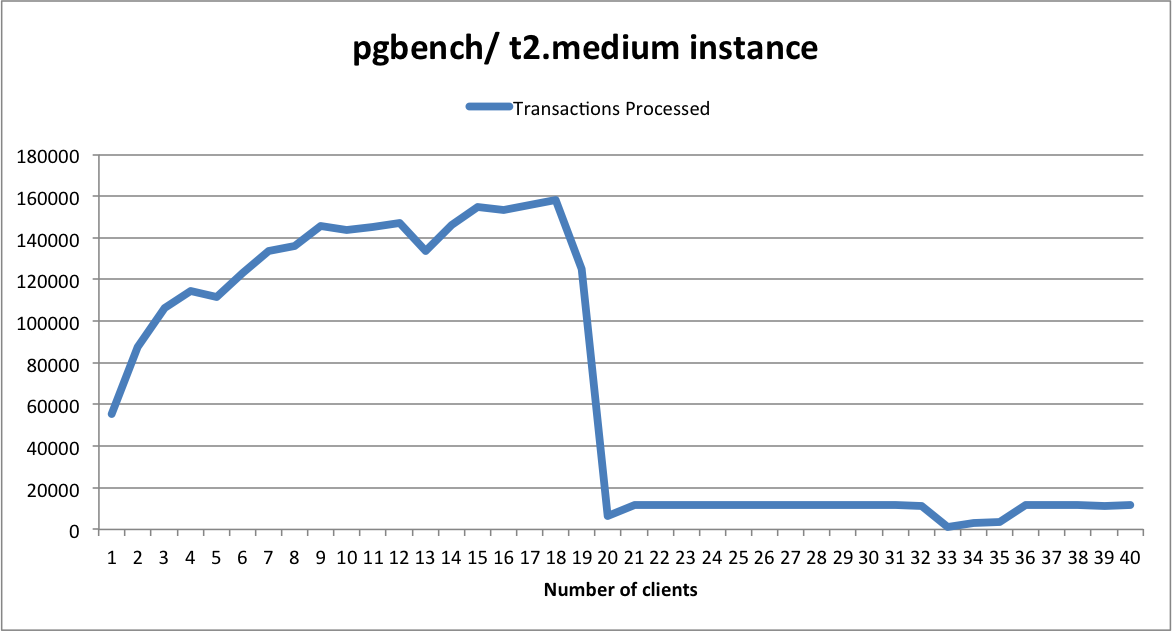
\includegraphics[scale=0.5]{pgbench.png}
	\caption{Database performance evaluation in a t2.medium amazon instance, increasing the number of clients in order to observe the maximum amount of transaction it can process.}
	\label{pgbench}
	%\input{soft-mmu-2.pdf}
\end{figure}
In order to have a first impression about database performance, and even before setting my own experiments to the messaging system. I decided to run some benchmarking tests in the database system.  In addition to get a good analysis of the performance of my database, the network time factor had to be removed. Therefore I decided to execute locally pgbench, which is a benchmarking tool, to find out the performance of my database.\\

The database server is a t2.medium instance of the amazon EC2, it has 2 vCPUs, 4GiB of Memory and it uses a 20 GB SSD for storage. The postgres database configuration is the following: max. number of connection is 100, it has a shared buffer of 120 MB. This is a basic postgres default configuration.\\	

For benchmarking pgbench has a default size configuration database with three tables, like the messaging systems. The normal size of the database is 15MB. However the size can scale with the scaling factor of pgbench. The number of rows in one of the pgbench tables is 100,000 and it grows with the scaling factor as well.\\

The benchmarking was performed for a three minutes period with different amount of clients in the database. The scaling factor of the benchmarking was of 100. 
As it is shown in Figure\ref{pgbench} the database achieves it maximal performance with 19 clients achieving a total of 124968 request, this database was loaded with concurrent request and with a scaling factor of 100. Therefore given load that the Messaging system can generate, its performance should not be affected at least by the database tier. This because this component can handle more load than the generated by the system.\\



\subsection{Middleware}\label{sec:middleware}

\subsubsection{Design overview}\label{sec:design-overview}
Overall the Middleware system has three main components, the Middleware server, the Client Handler and The Database Connector Server \( See Figure \ref{middle} \).
The Middleware server is main thread on the system. It is always listening to new connections from new clients. Before the running of the main listening connection socket the Middleware server sets up the connection with the database.\\

\begin{figure}[h!]
	\centering
	%\def \svgscale {\columnwidt}
	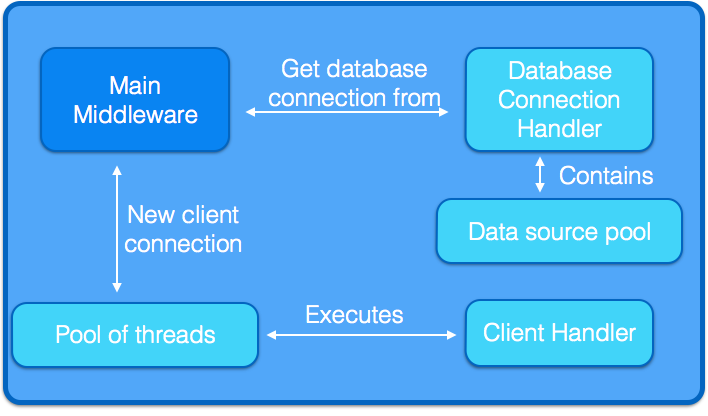
\includegraphics[scale=0.3]{midleware.png}
	\caption{Main middleware component schema.}
	\label{middle}
	%\input{soft-mmu-2.pdf}
\end{figure}


In order to establish this connection the Middleware needs the following parameters: the address of the database server, the port where the database is listening, the user to connect to the database, the password, the database’s name and finally the number of connection to handle. The latest parameter defines the behavior of the queuing of new incoming connections and the pool in the connection to the database; this behavior is explained more in detail in the Queuing and connection pool database section.\\
 
Whenever the middleware obtains a new connection from a new client, it pairs this connection with a socket and a connection to the database. The Database connector server gives the connection for the incoming user, after getting the connection a new thread from the Executor service in the Middleware is launched. The new thread takes the socket of the incoming connection and the connection to the database. The initial number of connections to handle limits the number of simultaneous threads in the Middleware.\\

The behavior of the executor service is explained more in details in further sections. The Client Handler is the component that is instantiated by the new thread in the executor service. Each thread of a Client Handler is in charge of a single user, therefore the system has a total number of handlers equal to the numbers of users been handle by the Middleware.\\

The Database Connection server:
Since the Middleware gets the parameters to enable the connection the database. It passes those parameters to the Database connection server in order to instantiate a new set of connections in a pool for the database.\\

The Client Handler:
This component of the middleware has all the logic to fulfill every request a client can do to the middleware. It uses the socket given by the Middleware to interact with the client and the database connection from the pool to interact with the database server. As result each client can successfully send messages and these will be stored in the database.


\subsubsection{Interfacing with clients}\label{sec:interfacing-with-clients}
The interface between users in the Middleware is the Client Handler. Nevertheless, the Client Handler uses a special object that helps during the interaction with the client. This is the Protocol component; it defines a message object, a queue object, a user object and a protocol number. The value on the protocol number defines the type of operation been requested by the user. The values and their corresponding protocol number are the one in Table\ref{opera}.\\

\begin{table}[h]\centering

\begin{tabular}
{|c|c|}
\hline  \textbf{Operation \#} & \textbf{Desciption} \\ 
\hline  99 & Initialize connection with client. \\ 
\hline  0 &  Read message from the queue.\\ 
\hline  1 &  Read message intended for the user.\\ 
\hline  2 &  Read message sent by a user.\\ 
\hline  3 &  Create a new message.\\ 
\hline  4 &  Create a new queue.\\ 
\hline  5 &  Send a message to a particular receiver.\\ 
\hline  6 &  Delete queue.\\ 
\hline  7 &  End connection \\ 
\hline 
\end{tabular} 
\caption{List of operations that can be performed by the client and their protocol number}
\label{opera}
\end{table}


\subsubsection{Queuing and Connection pool to database}\label{sec:queuing-and-connection-pool-to-database}
In the Middleware there are three queuing components: The Pool of executor in charge of executing a Client Handler per connection, the connection pool in charge of managing the connection to the database, and the queuing message system it self \( See Figure \ref{pool} \).\\

\begin{figure}[h!]
	\centering
	%\def \svgscale {\columnwidt}
	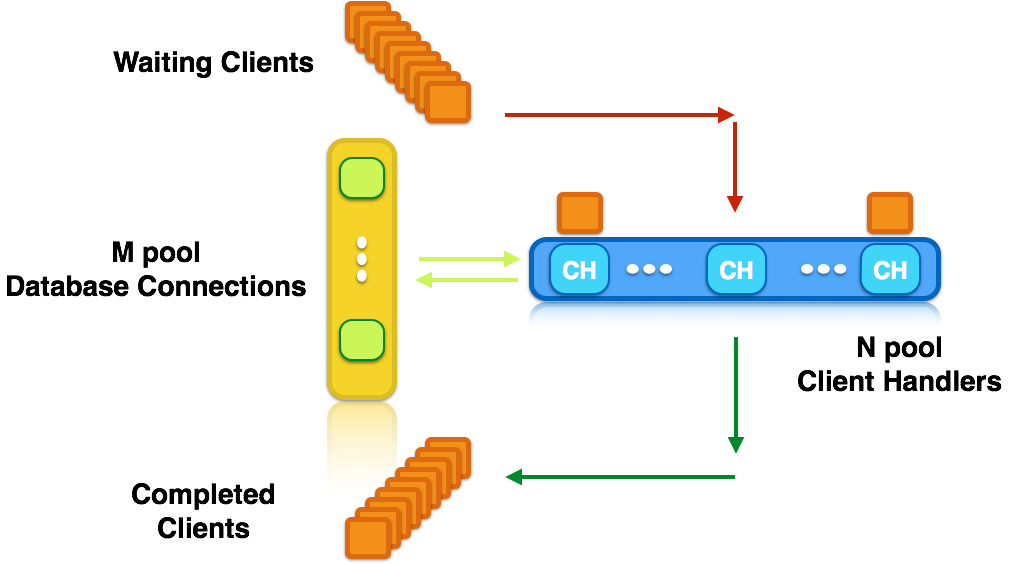
\includegraphics[scale=0.3]{connpool.png}
	\caption{Behavior of the system, M and N is the number of connection in each pool, the may be equal or different. The number of connections in the pool affects the througput in the system.}
	\label{pool}
	%\input{soft-mmu-2.pdf}
\end{figure}

The Executor service acts as a blocking queue. In this case this is a bounden queue since it has a maximum number of thread in this case is the number of users that it can handle concurrently. As part of the design of the system I wanted to use this technique in order to prevent resource starvation. When a system uses large queues and a relative small pools then the usage of the CPU and the OS resources, and the overhead due to context-switching decreases. Nevertheless this may also affect the throughput of the system.\\

The connection pool in charge of the connections has a fixed number of connections ready for the clients. Each connection is assigned to a Client Handler to interact with the request coming from the client. When a Client Handler is done with a client and it calls the closing method for the connection, this one never actually closes, instead it returns to the pool of connection in order to be used by another Client Handler. This improves the performance of the system, since there is no need to setup a new connection for new Client in the system.


\subsubsection{Performance characteristics}\label{sec:performance-characteristics-1}
Overall the evaluated metrics in the system are highly tied to the configuration of the system. A fixed set of parameters is considered a model and by changing a single parameter the systems becomes a completely different model with different throughput and response time.\\

In this system the metrics like the throughput correspond to the number of requests per second the middleware can handle. The type of request depends on the clients. The response time or latency is the time it takes to fulfill a request generated by the client, depending on where this is measured we can also have latency in the middleware and latency in the database.
In order to provide a description of the characteristics of the system, its parameters will be fixed in a specific setting describing normal use case of the system. \\

The system configuration consist of 5 machines from which 1 is the database machine, 2 are middleware nodes, and 2 are client machines running 30 clients each. The operation been performed by the clients is to send messages in the system. This behavior was decided in order to simulate a heavy operation situation of the system. This will give a clear description of the operation of the system under a stress condition. For this performance analysis the system has a single connection to the database and 30 handlers on each middleware node. This will show how the system react with a single connection been shared among the clients and how the performance affect the measured metrics for a period of 3 minutes.\\

Further on in the report other experiments where run, changing more values in certain parameters and behavior on the metrics differ.\\

In summary on middleware 1 the following result are found:\\
Total number of clients:	30\\
Average total of waiting time for all clients:	69.3144702642 ms\\
Average total of waiting time for all Client Handlers:	66.959272843 ms\\
Average Throughput in the Middleware:	465.727272727 req/s\\
Total \# of requests in Middleware:	128683\\
Utilization Law 	X=465.727272727	S=0.00213703441791 U=0.995275211178\\

 On middleware 2 we observe a almost equal behavior and this is because both have the same configuration:\\
Total number of clients:	30\\
Average total of waiting time for all clients:	68.8650415678 ms\\
Average total of waiting time for all Client Handlers:	66.8341319684 ms\\
Average Throughput in the Middleware:	472.386861314 req/s\\
Total \# of requests in Middleware:	129926\\
Utilization Law 	X=472.386861314	S=0.00210889275434	U=0.996213229069 \\

Overall on the system we had 60 clients and by summing both throughputs we a have a total of 938.1 requests per seconds with a latency of 68 ms this is including network delay time. In addition we can observe the system is being busy must of the time given the result on the utilization formula.\\

In this part for this performance results are merely presented on numbers. However detailed plots can be found in the experiment section.
The variations on results are result of the configuration of the main components affecting the system. Those are the queuing in the handlers pool, the connection pool of the database, the load in the system and the database. Nevertheless conclusions about each component are found on each experiment in the experiment section.


\subsection{Clients}\label{sec:clients}


\subsubsection{Design and interface}\label{sec:design-and-interface}

\begin{figure}[h!]
	\centering
	%\def \svgscale {\columnwidt}
	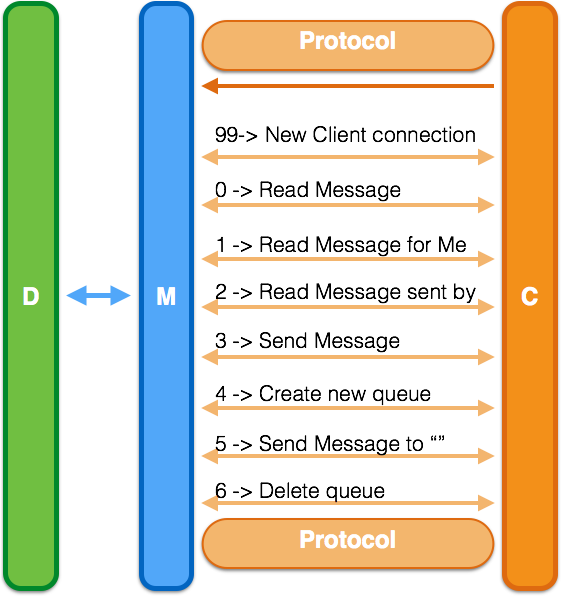
\includegraphics[scale=0.3]{prtocol.png}
	\caption{Client, middleware and database interaction procedure. This diagram show the operations that a client can request and the behavior between thr C:Client, M:Middleware and D:Database.}
	\label{interaction}
	%\input{soft-mmu-2.pdf}
\end{figure}
The design of the clients is simple. They accept different running modes, those are defined by the number of parameter they get during the running and deployment. The main parameters for running are the following: server address of the middleware, listening port of the middleware, and the client name. Once it starts running it can accept which operation to perform by console and fulfill the entire fields in the same manner. Nevertheless for experimenting purposes the clients are initialize with more parameter to avoid the interaction with a real user and automatize the operations that it performs. The extra parameter are the following: a running time that defines how long the clients are going to run, the workload under it will send a new request to the middleware, the operation number that is going to perform, this could be any of the ones defined in section \ref{sec:interfacing-with-clients}.\\

Furthermore inside each client there is embedded a single message with a length of 200 characters. The size of the message can change with a scaling parameter that is supplied during the launching moment in the client. This changing size feature is in the system since is defined in the system description. Additionally, they count with a list of pre-set user name and queue names from where they can choose randomly during the execution of certain client operations. (e.x. Sending a new message)  \( See Figure \ref{interaction} \).


\subsubsection{Instrumentation}\label{sec:instrumentation}

The instrumentation can be divided as the one added before compiling to the system and external tools used after running of the system. 
The clients in there source code, instrumentation logging mechanisms where added, in order to record data during running time, like throughput during unit time and records of the operations performed by it.\\

As external tools of instrumentation I used python script to parse the logs and perform all the measurements of my system. The scripts use the time stamp value of each of the operations logged in the log files. In addition to make an assumption about the time it takes the db to perform an operation a log entry is performed in the middleware level, in order to identify the log of the db a line in the log files has a db tag identifier which the parser is able to detect and use to estimate the database response time.\\

For details on how my instrumentation tools were used se the Workload and Deployment section. 


\subsubsection{Workloads and deployment}\label{sec:workloads-and-deployment}
 The workload behavior in the system is self-adjusting, since each client was not having a thinking time for sending a new request. In addition based on the design of system as a closed system, clients were not able to send more requests to the middleware if these ones where not having a response of the previous request. Therefor the load was based in the number of concurrent client being attended or served by the middleware. In addition the time between request was a consequence of the type of operation been requested, plus the time of processing by the middleware, network delay and time of processing in the database.\\
 \begin{figure}[h!]
 	\begin{boxedminipage}{\textwidth}
 	\tiny
 	\rule{\textwidth}{0.5pt}
 	\textsc{Exmaple of Deployment and Instrumentation Tools}\\
 	\rule{\textwidth}{0.5pt}
   Running The Experiment\\
   \#\  fab -R local fullAmazon1:experimentID=resp\_time\_1\_mid1\_cl5\_msg1,dbServer=52.30.174.216,dbName=messaging,dbUser=postgres,\\dbPassword=squirrel,noOfConnections=15,listeningPort=5432,noConnDB=5,duration=180,serverPort=5433,serverAddress=52.30.110.167,\\operationType=5,workload=0,noClients=15,messageType=1 \\
   
   Parsing the Results\\
   \#\ fab -R local parsing:pathOfLogs=/Users/pedrini/Documents/workspace/Middleware/script/logs\_exp\_resp\_time\_1\_mid1\_cl5\_msg1/
   
   Output Example\\
   Total number of clients:	15\\
   
   Average total of waiting time for all clients	36.2926324829\\
   Standard Deviation total of waiting time for all clients	0.44978481201\\
   Standard Error total of waiting time for all clients	0.120210047451\\
   
   Average total of waiting time for all Client Hanlders	34.5220723635\\
   Standard Deviation total of waiting time for all Client Hanlders	0.48504220643\\
   Standard Error total of waiting time for all Client Hanlders	0.129632982471\\
   
   
   Average Throughput in the Middleware:	438.239285714\\
   Standard Deviation of Throughput in the Middleware:	44.6265843199\\
   Standard Error of Throughput in the Middleware:	2.6717237184\\
   Total \#\ of requests in Middleware:	123226\\
   
   Utilization Law 	X=438.239285714	S=0.00227224773993	U=0.995788226511\\
  
   \end{boxedminipage}
   	\caption{Full run of experiment and parsing command}
   	\label{fig:deploy}
 \end{figure}
 
To deploy the system parameters as number of clients, operation performed by the clients, number of connections and size of messages were specified in the deployment scripts See Figure \ref{fig:deploy}. These scripts were described previously and were part of python instrumentation scripts used to parse and perform operations with the log resources.


\subsubsection{Sanity checks}\label{sec:sanity-checks}
The operation of sending new messages to the system is part of the sanity check of the system. For most of the experiments I started with and empty database. Therefore at the end of each experiment I was able to observe how many transaction my middleware was reporting. Once I got the number I performed a cross validation with the total number of live tuples in my database.\\
 
In addition giving the logs of the clients and the number of transactions they were reporting, the sum of the total of request of all the clients had to match the ones in the middleware. The python script performed these validations.
For checks regarding sensible operations in my system, like I/O error or connection errors the system has pertinent Exception handlers embedded. In addition if an error occur during the execution the system has a logger to register the error.\\

Furthermore to control transaction among client and middleware I implemented another sanity check tool which validates that each answer coming from the middleware correspond to the one requested by the client. If this not the case then the system trigger and alert on the logs.\\

Finally the construction is modular each critical component is well separated which allows a quick response time in case of a component fails. 
